% Build-vs-buy spectrum figure for Ch13 ("Build vs. Buy: Choosing a Harness").
% Standalone TikZ; compiled by `book-scaffold build-figures` via pdflatex -> pdftocairo -> SVG.
% A five-point spectrum from "direct on the API" to "build from scratch", with control
% rising left-to-right and maintenance cost rising with it. The recommended starting
% point is the left end; the configure/wrap/extend band is the dominant real-world answer.
\documentclass[tikz,border=4mm]{standalone}
\usepackage{tikz}
\usetikzlibrary{positioning, arrows.meta, calc, decorations.pathreplacing}

\begin{document}
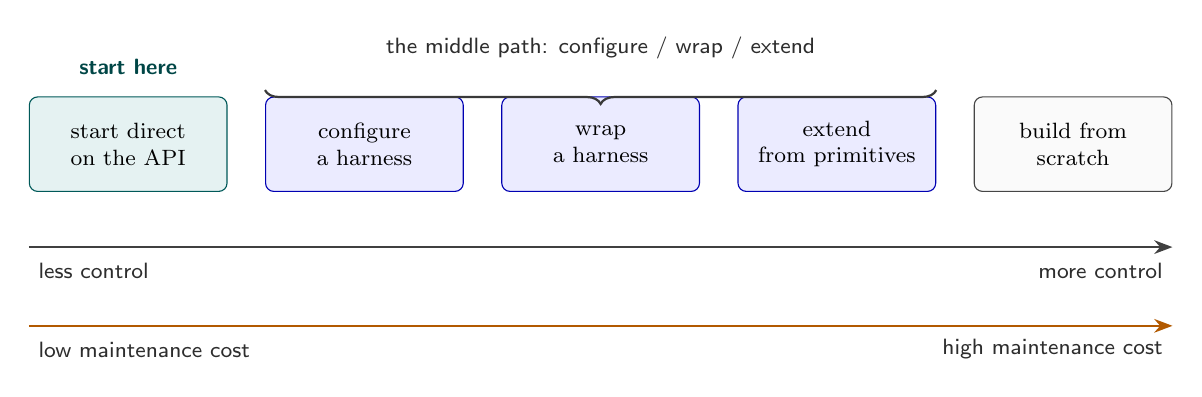
\begin{tikzpicture}[
  font=\sffamily,
  stage/.style={draw=gray!55!black, fill=gray!4, rounded corners=3pt, align=center,
    text width=2.3cm, minimum height=1.2cm, inner sep=3pt, font=\footnotesize},
  startbox/.style={draw=teal!70!black, fill=teal!10, rounded corners=3pt, align=center,
    text width=2.3cm, minimum height=1.2cm, inner sep=3pt, font=\footnotesize},
  midbox/.style={draw=blue!70!black, fill=blue!8, rounded corners=3pt, align=center,
    text width=2.3cm, minimum height=1.2cm, inner sep=3pt, font=\footnotesize},
  ax/.style={-Stealth, thick, draw=gray!50!black},
  caplbl/.style={font=\sffamily\footnotesize, text=gray!35!black}
]

% The five stages, left to right.
\node[startbox] (s0) at (0,0)   {start direct\\on the API};
\node[midbox]   (s1) at (3,0)   {configure\\a harness};
\node[midbox]   (s2) at (6,0)   {wrap\\a harness};
\node[midbox]   (s3) at (9,0)   {extend\\from primitives};
\node[stage]    (s4) at (12,0)  {build from\\scratch};

% the middle band annotation
\draw[decorate, decoration={brace, amplitude=5pt, raise=2pt}, gray!45!black, thick]
  ($(s3.north east)+(0,0.15)$) -- ($(s1.north west)+(0,0.15)$);
\node[caplbl, anchor=south] at ($(s2.north)+(0,0.35)$)
  {the middle path: configure / wrap / extend};

% control axis (rises left to right)
\draw[ax] (s0.south west)+(0,-0.7) -- ($(s4.south east)+(0,-0.7)$)
  node[midway, below=2pt, font=\sffamily\bfseries, text=blue!55!black] {};
\node[caplbl, anchor=west] at ($(s0.south west)+(0,-1.0)$) {less control};
\node[caplbl, anchor=east] at ($(s4.south east)+(0,-1.0)$) {more control};

% maintenance-cost axis (also rises left to right)
\draw[ax, draw=orange!70!black] ($(s0.south west)+(0,-1.7)$) -- ($(s4.south east)+(0,-1.7)$);
\node[caplbl, anchor=west] at ($(s0.south west)+(0,-2.0)$) {low maintenance cost};
\node[caplbl, anchor=east] at ($(s4.south east)+(0,-2.0)$) {high maintenance cost};

% the recommended-start marker
\node[font=\sffamily\bfseries\footnotesize, text=teal!55!black, anchor=south]
  at ($(s0.north)+(0,0.15)$) {start here};

\end{tikzpicture}
\end{document}
